% Phylgrowth User Guide
%
% For PDF output: pdflatex phylogrowth.tex
% For HTML output: plastex pyhlogrowth.tex
%
% For Graphics:
% Use PNG format to avoid problems with HTML conversion.
% Recommended size: < 13cm x 18cm (width x height).
% Recommended resolution: 300 dpi.
%
% Use fixed width instead of textwidth, so that plastex can
% recognize the graphics size. For example use
% \includegraphics[width=13cm]{img/haplogroups.png}
% instead of
% \includegraphics[width=\textwidth]{img/haplogroups.png}


\documentclass[12pt,a4paper]{article}
\usepackage[utf8]{inputenc}
\usepackage[russian,english]{babel}
\usepackage[colorlinks=true, urlcolor=blue, linkcolor=blue]{hyperref}
\usepackage{graphicx}

\begin{document}
\begin{titlepage}

\title{Phylogrowth User Guide}

\author{Dirk Struve\\
phylofriend at projectory.de\\
\href{https://github.com/yogischogi/phylogrowth/}{https://github.com/yogischogi/phylogrowth/}}
\date{\today}
\end{titlepage}
\maketitle

\tableofcontents
\section{Introduction}

Phylogrowth is a program that calculates population growth
from a phylogenetic tree by counting subclades and samples
for given periods of time.

Periods of human growth and prosperity are often accompanied
by strong population growth. For a society strong population
growth simply means more surviving children. If more children
survive there is also a higher chance of more mutations and
thus more new branches on the phylogenetic tree. So a high
number of new branches within a given period of time indicates
strong population growth and good times.

Population growth usually continues until resources get scarce
or the society is threatened by epidemics, natural disasters or
war. It should be possible to detect those times by looking at
the population growth.

Luckily we all carry important archeological evidence within us.
It is encoded in our genetic markers. Modern technologies like
next generation sequencing have made it possible to create highly
accurate phylogenetic trees.

Phylogrowth can utilize those trees and give us insights into
our history.


\vspace{1em}\noindent
Have fun exploring human history!

\vspace{1em} Dirk




\section{Installation}

This guide is mainly targeted towards persons who use Linux Mint
or other Linux versions of the Debian family. Some familiarity
with the use of Linux commands is assumed.

Currently there are no binary distributions available for
Windows or the Mac. Users of these operating systems can
use Phylogrowth as well, but they will experience some
laborious installation work. The best way is to follow the
instructions provided on the
\href{http://golang.org/}{Go} home page.

The following list applies to Linux users only:

\begin{enumerate}
\item Make sure that the Go programming language is installed.
	If not it can be installed by typing\\
	\texttt{sudo apt-get install golang}
\item Read the Go
	\href{http://golang.org/doc/install}{Getting Started}
	guide. Make sure to set your \emph{GOPATH} variable and
	include it in your \emph{PATH} so that Go programs can be
	found.
\item Fetch the Phylogrowth program with\\
	\texttt{go get github.com/yogischogi/phylogrowth}
\item Install the program with\\
	 \texttt{go install github.com/yogischogi/phylogrowth}
\end{enumerate}

Now the Phylogrowth program should be installed.


\section{Command Line Options}

Command line options may be given in arbitrary order.
Parameters may be specified by using a space or equals sign.
For example the following options are identical:
\texttt{-treein=mytree}, \texttt{-treein mytree}.

\begin{description}
\item[-help] Prints available program options.

\item[-treein] Input filename for phylogenetic tree (.txt).
\item[-treeout] Output filename for phylogenetic tree in TXT format.
\item[-csvout] Output filename for histogram data in CSV format.
\item[-txtout] Output filename for histogram data in TXT format.
\item[-pngout] Output filename for PNG image.
	 Needs Gnuplot \cite{Gnuplot} to be installed.
\item[-step] Step length of histogram intervals in years.
	Default is 100.
\item[-subclade] Selects a specific branch of the tree.
\end{description}


\section{Examples}

\subsection{First Steps}

\subsubsection*{Phylogenetic Input Tree}

Before you can start you need to create a phylogenetic tree,
that contains SNPs, IDs of the genetic samples and TMRCA
estimates. The file format is text based and looks like this:

\begin{verbatim}
// This is an example tree.
// Comments begin with //.

CTS4528, S1200 TMRCA 5000
    S11481 TMRCA 2000
        id:YF01234
        id:YF00301
        id:YF02016
    S14328 TMRCA 4500
        id:YF04242
        id:YF00101
        id:YF01010
\end{verbatim}

Each line of the tree contains one or more SNPs or a sample
ID. Subclades and samples are indented by using tabs or spaces.
Each sample starts with \texttt{id:} followed by the ID.

If a subclade has a TMRCA estimate Phylogrowth counts the number
of additional new lineages. As a first rough estimate we assume
that the number of new lineages is proportional to population
growth.

To create a graph that shows the new lineages from the example
tree:

\begin{enumerate}
\item Save the example tree to a file, for example \emph{tree.txt}.
\item Go to a command line and type:\\
	\texttt{phylogrowth -treein=tree.txt -pngout=example.png}\\
	For this to work you need Gnuplot \cite{Gnuplot} to be installed.
\item Done! Your first graph should be stored in the file \emph{example.png}.
\end{enumerate}

\begin{figure}[ht]
\centering
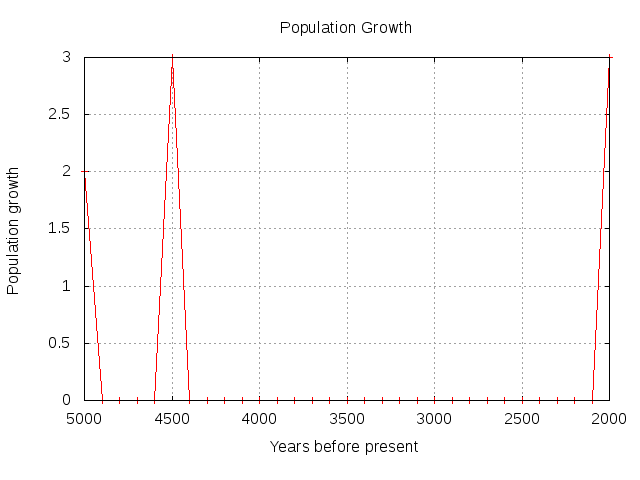
\includegraphics[width=13cm]{img/example.png}
\caption{The first example showing time periods of haplogroup
expansion.}
\end{figure}

\pagebreak


\subsection{Using the YFull Tree}

Phylogrowth is especially well suited for the use of the YFull
tree \cite{YFullTree}. It's TMRCA estimates are based on SNP
counting and calibrated by ancient and modern DNA samples
\cite{YFullMutationRate}.

As a more sophisticated example let us calculate the number of
new lineages for the P312 haplogroup. P312 is widespread in Western
Europe and most common in Spain, France and on the British Isles.

\begin{enumerate}
\item Go to the YFull R1b tree at
	\href{https://yfull.com/tree/R1b/}{https://yfull.com/tree/R1b/}.
\item Copy the tree directly from the Web page and save it
	to a text file named \emph{yfull-tree.txt}.
	Be careful that the indentations are preserved.
\item Go to a command line and type:\\
	\texttt{phylogrowth -treein=yfull-tree.txt -subclade=P312 -pngout=P312.png}
\item Done! Now watch \emph{P312.png}. Can you spot the Bronze Age
	expansion, the Roman Empire and the Migration Period?
\end{enumerate}


\begin{figure}[ht]
\centering
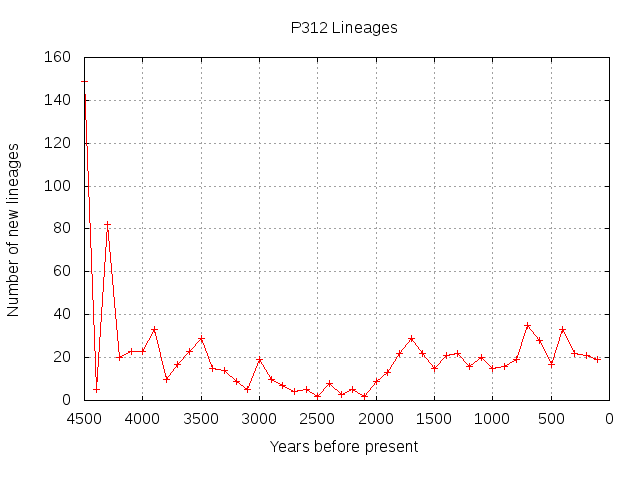
\includegraphics[width=13cm]{img/P312.png}
\caption{Number of new lineages of the P312 haplogroup.}
\end{figure}







\section{Theory}

\subsection{Population Growth}

Let us assume that we have a closed population and take a
number of genetic samples. We analyse the samples and get
different genetic lineages as a result.

The number of genetic lineages is proportional to the 
total population size.

\begin{equation}
L \sim P \label{lineages-population}
\end{equation}

\begin{tabular}{ll}
L:   & number of detected lineages\\
P:   & population size
\end{tabular}
\vspace{1em}

If we detect all male lineages, for example, the population
size would be about twice as much.

How does population size change with time? If we look after a
short period of time we may take the old population size, add
the number of births and subtract the number of deaths.

\begin{equation}
P(t+dt) = P(t) + b(t)dt - d(t)dt 
\end{equation}

\begin{tabular}{ll}
$P$: & population size\\
$b$: & number of births per second\\
$d$: & number of deaths per second\\
$t$: &time
\end{tabular}
\vspace{1em}

The probability of a mutation is the same for all newborn
babies. This means the number of newly appearing mutations
and lineages within a period of time scales with the number
of births within that period. Thus we are interested in the
number of births and rewrite the previous formula as

\begin{equation}
b(t)dt = P(t+dt) - P(t) + d(t)dt
\end{equation}

or

\begin{eqnarray}
b(t) & = & \frac{P(t+dt)- P(t)}{dt} + d(t)\\
     & = & \frac{dP(t)}{dt} + d(t) \label{births-per-second}
\end{eqnarray}

As an easy model let us assume that the number of deaths
per second is proportional to the total population size.
In this case the following equation holds:

\begin{equation}
d(t) = c_{d} P(t)
\end{equation}

\begin{tabular}{ll}
$d$:     & number of deaths per second\\
$P$:     & population size\\
$c_{d}$: & constant
\end{tabular}
\vspace{1em}

Under this assumption we can rewrite equation \ref{births-per-second}
as

\begin{equation}
b(t) = \frac{dP(t)}{dt} + c_{d} P(t)
\label{births-per-second-final}
\end{equation}

This means that the number of births per second depends on
two terms, the population growth and the population size.


\subsection{Measurement of Phylogenetic Growth}

We can not measure the number of births for every point in
history directly. We can only look at a phylogenetic tree
and examine how the number of lineages increases with time.

Let us assume that a fraction $c_l$ of all births develops
into lineages that are still on the phylogenetic tree today.
If we try to count these lineages we can count all new lineages
on the phylogenetic tree between to points in time.

\begin{equation}
g(t) = c_l \int\limits_{t-\frac{a}{2}}^{t+\frac{a}{2}} b(t) dt
\end{equation}

If we substitute $b(t)$ with equation \ref{births-per-second-final}
we get

\begin{equation}
g(t) = c_l \int\limits_{t-\frac{a}{2}}^{t+\frac{a}{2}} \frac{dP(t)}{dt} + c_{d} P(t) dt
\end{equation}

\begin{tabular}{ll}
$g$:     & growth of phylogenetic lineages between $t-\frac{a}{2}$ and $t+\frac{a}{2}$\\
$a$:     & time interval or step length used for counting\\
$c_l$:   & fraction of births that develops into long time lineages\\
$P$:     & population size\\
$c_{d}$: & fraction of the population size that dies per second
\end{tabular}
\vspace{1em}

For practical purposes we assume that the measurement time
interval $a$ is small compared to the time it takes for any
significant population changes. Then we may write the previous
equation as

\begin{equation}
g(t) \approx c_l a \left( \frac{dP(t)}{dt} + c_{d} P(t) \right) \label{phylogrowth}
\end{equation}

This means that the measured increase in phylogenetic lineages
at any given time is roughly proportional to the number of births
at that time and this depends on population size and growth.

Equation \ref{phylogrowth} is only valid for complete phylogenetic
trees. In reality we have to take into account that only a fraction
$c_t$ of the population has tested.

Furthermore the probability to detect a certain lineage depends
on it's age. If we characterize a specific historic lineage by
it's SNP mutation we will find this mutation whenever a person
belonging to the SNP subclade has tested. Thus the probability
to detect a certain SNP scales with the number of persons
carrying it. For simplicity we assume that all subclades grow
equally with population growth.

If the fraction $c_t$ of the population that has tested is
very small, we will miss most of the younger lineages. The
older ones however will be amplified by the number of their
sublineages and thus population growth.
In this case we may write:

\begin{eqnarray}
d(t) & \approx & c_t \frac{P(t_0)}{P(t)} g(t)\\
     & \approx & c_t \frac{P(t_0)}{P(t)} c_l a b(t) \\
     & \approx & c_t \frac{P(t_0)}{P(t)} c_l a \left( \frac{dP(t)}{dt} + c_{d} P(t) \right)
\end{eqnarray}

\begin{tabular}{ll}
$d$:     & detected number of new lineages between $t-\frac{a}{2}$ and $t+\frac{a}{2}$\\
$c_t$:   & fraction of the population that has tested.\\
$P$:     & population size\\
$t$:     & time\\
$t_0$:   & time of testing\\
$g$:     & growth of phylogenetic lineages between $t-\frac{a}{2}$ and $t+\frac{a}{2}$\\
$b$:     & number of births per second\\
$a$:     & time interval or step length used for counting\\
$c_l$:   & fraction of births that develops into long time lineages\\
$c_{d}$: & fraction of the population size that dies per second
\end{tabular}
\vspace{1em}












\raggedright
\begin{thebibliography}{bla}

\bibitem{YFullMutationRate} Dmitry Adamov, Vladimir Guryanov,
Sergey Karzhavin, Vladimir Tagankin, Vadim Urasin.
\emph{\href{http://rjgg.molgen.org/index.php/RJGGRE/article/view/151}
{Defining a New Rate Constant for Y-Chromosome SNPs based on Full Sequencing Data}}.
The Russian Journal of Genetic Genealogy
(\foreignlanguage{russian}{Русская версия}),
Vol 6, No 2 (2014)/Vol 7, No 1 (2015).

\bibitem{Gnuplot} Thomas Williams, Colin Kelley,
\emph{\href{http://www.gnuplot.info/}{Gnuplot}}.
Thomas Williams, Colin Kelley, 1986--1993, 1998, 2004,
Date visited: 2016-06-23.

\bibitem{YFullTree} YFull,
\emph{\href{http://yfull.com/tree/}{YFull Phylogenetic Tree}}.
Date visited: 2016-06-23.


\end{thebibliography}

\bibliography{references}
\addcontentsline{toc}{section}{References}
\end{document}
